\documentclass[twoside]{book}

% Packages required by doxygen
\usepackage{fixltx2e}
\usepackage{calc}
\usepackage{doxygen}
\usepackage[export]{adjustbox} % also loads graphicx
\usepackage{graphicx}
\usepackage[utf8]{inputenc}
\usepackage{makeidx}
\usepackage{multicol}
\usepackage{multirow}
\PassOptionsToPackage{warn}{textcomp}
\usepackage{textcomp}
\usepackage[nointegrals]{wasysym}
\usepackage[table]{xcolor}

% Font selection
\usepackage[T1]{fontenc}
\usepackage[scaled=.90]{helvet}
\usepackage{courier}
\usepackage{amssymb}
\usepackage{sectsty}
\renewcommand{\familydefault}{\sfdefault}
\allsectionsfont{%
  \fontseries{bc}\selectfont%
  \color{darkgray}%
}
\renewcommand{\DoxyLabelFont}{%
  \fontseries{bc}\selectfont%
  \color{darkgray}%
}
\newcommand{\+}{\discretionary{\mbox{\scriptsize$\hookleftarrow$}}{}{}}

% Page & text layout
\usepackage{geometry}
\geometry{%
  a4paper,%
  top=2.5cm,%
  bottom=2.5cm,%
  left=2.5cm,%
  right=2.5cm%
}
\tolerance=750
\hfuzz=15pt
\hbadness=750
\setlength{\emergencystretch}{15pt}
\setlength{\parindent}{0cm}
\setlength{\parskip}{3ex plus 2ex minus 2ex}
\makeatletter
\renewcommand{\paragraph}{%
  \@startsection{paragraph}{4}{0ex}{-1.0ex}{1.0ex}{%
    \normalfont\normalsize\bfseries\SS@parafont%
  }%
}
\renewcommand{\subparagraph}{%
  \@startsection{subparagraph}{5}{0ex}{-1.0ex}{1.0ex}{%
    \normalfont\normalsize\bfseries\SS@subparafont%
  }%
}
\makeatother

% Headers & footers
\usepackage{fancyhdr}
\pagestyle{fancyplain}
\fancyhead[LE]{\fancyplain{}{\bfseries\thepage}}
\fancyhead[CE]{\fancyplain{}{}}
\fancyhead[RE]{\fancyplain{}{\bfseries\leftmark}}
\fancyhead[LO]{\fancyplain{}{\bfseries\rightmark}}
\fancyhead[CO]{\fancyplain{}{}}
\fancyhead[RO]{\fancyplain{}{\bfseries\thepage}}
\fancyfoot[LE]{\fancyplain{}{}}
\fancyfoot[CE]{\fancyplain{}{}}
\fancyfoot[RE]{\fancyplain{}{\bfseries\scriptsize Generated by Doxygen }}
\fancyfoot[LO]{\fancyplain{}{\bfseries\scriptsize Generated by Doxygen }}
\fancyfoot[CO]{\fancyplain{}{}}
\fancyfoot[RO]{\fancyplain{}{}}
\renewcommand{\footrulewidth}{0.4pt}
\renewcommand{\chaptermark}[1]{%
  \markboth{#1}{}%
}
\renewcommand{\sectionmark}[1]{%
  \markright{\thesection\ #1}%
}

% Indices & bibliography
\usepackage{natbib}
\usepackage[titles]{tocloft}
\setcounter{tocdepth}{3}
\setcounter{secnumdepth}{5}
\makeindex

% Hyperlinks (required, but should be loaded last)
\usepackage{ifpdf}
\ifpdf
  \usepackage[pdftex,pagebackref=true]{hyperref}
\else
  \usepackage[ps2pdf,pagebackref=true]{hyperref}
\fi
\hypersetup{%
  colorlinks=true,%
  linkcolor=blue,%
  citecolor=blue,%
  unicode%
}

% Custom commands
\newcommand{\clearemptydoublepage}{%
  \newpage{\pagestyle{empty}\cleardoublepage}%
}

\usepackage{caption}
\captionsetup{labelsep=space,justification=centering,font={bf},singlelinecheck=off,skip=4pt,position=top}

%===== C O N T E N T S =====

\begin{document}

% Titlepage & ToC
\hypersetup{pageanchor=false,
             bookmarksnumbered=true,
             pdfencoding=unicode
            }
\pagenumbering{alph}
\begin{titlepage}
\vspace*{7cm}
\begin{center}%
{\Large My Project }\\
\vspace*{1cm}
{\large Generated by Doxygen 1.8.13}\\
\end{center}
\end{titlepage}
\clearemptydoublepage
\pagenumbering{roman}
\tableofcontents
\clearemptydoublepage
\pagenumbering{arabic}
\hypersetup{pageanchor=true}

%--- Begin generated contents ---
\chapter{Class Index}
\doxysection{Class List}
Here are the classes, structs, unions and interfaces with brief descriptions\+:\begin{DoxyCompactList}
\item\contentsline{section}{\mbox{\hyperlink{structgrille}{grille}} }{\pageref{structgrille}}{}
\end{DoxyCompactList}

\chapter{File Index}
\section{File List}
Here is a list of all documented files with brief descriptions\+:\begin{DoxyCompactList}
\item\contentsline{section}{include/\hyperlink{grille_8h}{grille.\+h} }{\pageref{grille_8h}}{}
\item\contentsline{section}{include/\hyperlink{io_8h}{io.\+h} }{\pageref{io_8h}}{}
\item\contentsline{section}{include/\hyperlink{jeu_8h}{jeu.\+h} }{\pageref{jeu_8h}}{}
\end{DoxyCompactList}

\chapter{Class Documentation}
\hypertarget{structgrille}{}\doxysection{grille Struct Reference}
\label{structgrille}\index{grille@{grille}}
\doxysubsection*{Public Attributes}
\begin{DoxyCompactItemize}
\item 
\mbox{\Hypertarget{structgrille_a0b4da1e205825df205b0c004d105d62a}\label{structgrille_a0b4da1e205825df205b0c004d105d62a}} 
int {\bfseries nbl}
\item 
\mbox{\Hypertarget{structgrille_a48d6706d41bee6fff9200d872b8b0cd0}\label{structgrille_a48d6706d41bee6fff9200d872b8b0cd0}} 
int {\bfseries nbc}
\item 
\mbox{\Hypertarget{structgrille_a428cf0c0297ce04e0206ba0067ac3b42}\label{structgrille_a428cf0c0297ce04e0206ba0067ac3b42}} 
int $\ast$$\ast$ {\bfseries cellules}
\end{DoxyCompactItemize}
\doxysubsection*{Related Functions}
(Note that these are not member functions.) \begin{DoxyCompactItemize}
\item 
void \mbox{\hyperlink{structgrille_ae621f51c60aa4fafaa0c9f6c9b5a4036}{alloue\+\_\+grille}} (int l, int c, \mbox{\hyperlink{structgrille}{grille}} $\ast$g)
\item 
void \mbox{\hyperlink{structgrille_a7074b2b15576e9d2b3cd15c3a1dc7012}{libere\+\_\+grille}} (\mbox{\hyperlink{structgrille}{grille}} $\ast$g)
\item 
void \mbox{\hyperlink{structgrille_adf5501cc0bbad28f5ffc561d92197e4e}{init\+\_\+grille\+\_\+from\+\_\+file}} (char $\ast$filename, \mbox{\hyperlink{structgrille}{grille}} $\ast$g)
\item 
static void \mbox{\hyperlink{structgrille_a32d986d81f64f5bf9a58653accac0310}{set\+\_\+vivante}} (int i, int j, \mbox{\hyperlink{structgrille}{grille}} g)
\item 
static void \mbox{\hyperlink{structgrille_a9e6ec43aa272ad177a8b76aa2908bc18}{set\+\_\+non\+\_\+viable}} (int i, int j, \mbox{\hyperlink{structgrille}{grille}} g)
\item 
static int \mbox{\hyperlink{structgrille_a6abb75941488a79e824ca42165d1d8e9}{est\+\_\+non\+\_\+viable}} (int i, int j, \mbox{\hyperlink{structgrille}{grille}} g)
\item 
static void \mbox{\hyperlink{structgrille_a10e7b11f2de74ccf95ad1fcb3671a163}{set\+\_\+morte}} (int i, int j, \mbox{\hyperlink{structgrille}{grille}} g)
\item 
static int \mbox{\hyperlink{structgrille_aac3db82b0f857dc49ccd51628cbc231b}{est\+\_\+vivante}} (int i, int j, \mbox{\hyperlink{structgrille}{grille}} g)
\item 
void \mbox{\hyperlink{structgrille_a63b3ae16c86b568f6aa8f9ce84128b1e}{copie\+\_\+grille}} (\mbox{\hyperlink{structgrille}{grille}} gs, \mbox{\hyperlink{structgrille}{grille}} gd)
\item 
int \mbox{\hyperlink{structgrille_a43ff0b44e98c40583c0f2c154747464b}{oscillante}} (\mbox{\hyperlink{structgrille}{grille}} ga, \mbox{\hyperlink{structgrille}{grille}} gcop, int col)
\item 
void \mbox{\hyperlink{structgrille_a40f511f71c752cf84d0ddd91fae3aaff}{affiche\+\_\+grille}} (\mbox{\hyperlink{structgrille}{grille}} g, int v)
\item 
void \mbox{\hyperlink{structgrille_ab36a6f8957cd3e682119007836ce6ad5}{efface\+\_\+grille}} (\mbox{\hyperlink{structgrille}{grille}} g)
\item 
void \mbox{\hyperlink{structgrille_a88493b3c55828670e47150a95ed7db5b}{debut\+\_\+jeu}} (\mbox{\hyperlink{structgrille}{grille}} $\ast$g, \mbox{\hyperlink{structgrille}{grille}} $\ast$gc)
\item 
void \mbox{\hyperlink{structgrille_ac6106c698b8428f760e210c1aac40976}{vieillissement}} (\mbox{\hyperlink{structgrille}{grille}} $\ast$g, \mbox{\hyperlink{structgrille}{grille}} $\ast$gc)
\item 
int \mbox{\hyperlink{structgrille_a133fec89dff5c83e758f92ae02702bc5}{compte\+\_\+voisins\+\_\+vivants\+\_\+non\+\_\+cycl}} (int i, int j, \mbox{\hyperlink{structgrille}{grille}} g)
\item 
int \mbox{\hyperlink{structgrille_ac60adde70a78a7c05b88e9e8c0caaf6f}{compte\+\_\+voisins\+\_\+vivants\+\_\+cycl}} (int i, int j, \mbox{\hyperlink{structgrille}{grille}} g)
\item 
void \mbox{\hyperlink{structgrille_a370aeae582cd5114e64468c82b394c15}{evolue}} (\mbox{\hyperlink{structgrille}{grille}} $\ast$g, \mbox{\hyperlink{structgrille}{grille}} $\ast$gc, int($\ast$compte\+\_\+voisins\+\_\+vivants)(int, int, \mbox{\hyperlink{structgrille}{grille}}), int vj)
\end{DoxyCompactItemize}


\doxysubsection{Friends And Related Function Documentation}
\mbox{\Hypertarget{structgrille_a40f511f71c752cf84d0ddd91fae3aaff}\label{structgrille_a40f511f71c752cf84d0ddd91fae3aaff}} 
\index{grille@{grille}!affiche\_grille@{affiche\_grille}}
\index{affiche\_grille@{affiche\_grille}!grille@{grille}}
\doxysubsubsection{\texorpdfstring{affiche\_grille()}{affiche\_grille()}}
{\footnotesize\ttfamily void affiche\+\_\+grille (\begin{DoxyParamCaption}\item[{\mbox{\hyperlink{structgrille}{grille}}}]{g,  }\item[{int}]{v }\end{DoxyParamCaption})\hspace{0.3cm}{\ttfamily [related]}}

affiche une grille


\begin{DoxyParams}{Parameters}
{\em g} & grille g \\
\hline
{\em v} & toggle vieillisement \\
\hline
\end{DoxyParams}
\begin{DoxyReturn}{Returns}
{\ttfamily void} 
\end{DoxyReturn}
\mbox{\Hypertarget{structgrille_ae621f51c60aa4fafaa0c9f6c9b5a4036}\label{structgrille_ae621f51c60aa4fafaa0c9f6c9b5a4036}} 
\index{grille@{grille}!alloue\_grille@{alloue\_grille}}
\index{alloue\_grille@{alloue\_grille}!grille@{grille}}
\doxysubsubsection{\texorpdfstring{alloue\_grille()}{alloue\_grille()}}
{\footnotesize\ttfamily void alloue\+\_\+grille (\begin{DoxyParamCaption}\item[{int}]{l,  }\item[{int}]{c,  }\item[{\mbox{\hyperlink{structgrille}{grille}} $\ast$}]{g }\end{DoxyParamCaption})\hspace{0.3cm}{\ttfamily [related]}}

alloue une grille


\begin{DoxyParams}{Parameters}
{\em l} & nombre de lignes \\
\hline
{\em c} & nombre de colonnes \\
\hline
{\em g} & grille a allouer \\
\hline
\end{DoxyParams}
\begin{DoxyReturn}{Returns}
{\ttfamily void} 
\end{DoxyReturn}
\mbox{\Hypertarget{structgrille_ac60adde70a78a7c05b88e9e8c0caaf6f}\label{structgrille_ac60adde70a78a7c05b88e9e8c0caaf6f}} 
\index{grille@{grille}!compte\_voisins\_vivants\_cycl@{compte\_voisins\_vivants\_cycl}}
\index{compte\_voisins\_vivants\_cycl@{compte\_voisins\_vivants\_cycl}!grille@{grille}}
\doxysubsubsection{\texorpdfstring{compte\_voisins\_vivants\_cycl()}{compte\_voisins\_vivants\_cycl()}}
{\footnotesize\ttfamily int compte\+\_\+voisins\+\_\+vivants\+\_\+cycl (\begin{DoxyParamCaption}\item[{int}]{i,  }\item[{int}]{j,  }\item[{\mbox{\hyperlink{structgrille}{grille}}}]{g }\end{DoxyParamCaption})\hspace{0.3cm}{\ttfamily [related]}}

compte le nombre de voisins


\begin{DoxyParams}{Parameters}
{\em i} & nombre de lignes \\
\hline
{\em j} & nombre de colonnes \\
\hline
\end{DoxyParams}
\begin{DoxyReturn}{Returns}
{\ttfamily int} 
\end{DoxyReturn}
\mbox{\Hypertarget{structgrille_a133fec89dff5c83e758f92ae02702bc5}\label{structgrille_a133fec89dff5c83e758f92ae02702bc5}} 
\index{grille@{grille}!compte\_voisins\_vivants\_non\_cycl@{compte\_voisins\_vivants\_non\_cycl}}
\index{compte\_voisins\_vivants\_non\_cycl@{compte\_voisins\_vivants\_non\_cycl}!grille@{grille}}
\doxysubsubsection{\texorpdfstring{compte\_voisins\_vivants\_non\_cycl()}{compte\_voisins\_vivants\_non\_cycl()}}
{\footnotesize\ttfamily int compte\+\_\+voisins\+\_\+vivants\+\_\+non\+\_\+cycl (\begin{DoxyParamCaption}\item[{int}]{i,  }\item[{int}]{j,  }\item[{\mbox{\hyperlink{structgrille}{grille}}}]{g }\end{DoxyParamCaption})\hspace{0.3cm}{\ttfamily [related]}}

compte le nombre de voisins


\begin{DoxyParams}{Parameters}
{\em i} & nombre de lignes \\
\hline
{\em j} & nombre de colonnes \\
\hline
\end{DoxyParams}
\begin{DoxyReturn}{Returns}
{\ttfamily int} 
\end{DoxyReturn}
\mbox{\Hypertarget{structgrille_a63b3ae16c86b568f6aa8f9ce84128b1e}\label{structgrille_a63b3ae16c86b568f6aa8f9ce84128b1e}} 
\index{grille@{grille}!copie\_grille@{copie\_grille}}
\index{copie\_grille@{copie\_grille}!grille@{grille}}
\doxysubsubsection{\texorpdfstring{copie\_grille()}{copie\_grille()}}
{\footnotesize\ttfamily void copie\+\_\+grille (\begin{DoxyParamCaption}\item[{\mbox{\hyperlink{structgrille}{grille}}}]{gs,  }\item[{\mbox{\hyperlink{structgrille}{grille}}}]{gd }\end{DoxyParamCaption})\hspace{0.3cm}{\ttfamily [related]}}

recopie une grille dans une autre


\begin{DoxyParams}{Parameters}
{\em gs} & grille recopié \\
\hline
{\em gd} & grille affecté \\
\hline
\end{DoxyParams}
\begin{DoxyReturn}{Returns}
{\ttfamily void} 
\end{DoxyReturn}
\mbox{\Hypertarget{structgrille_a88493b3c55828670e47150a95ed7db5b}\label{structgrille_a88493b3c55828670e47150a95ed7db5b}} 
\index{grille@{grille}!debut\_jeu@{debut\_jeu}}
\index{debut\_jeu@{debut\_jeu}!grille@{grille}}
\doxysubsubsection{\texorpdfstring{debut\_jeu()}{debut\_jeu()}}
{\footnotesize\ttfamily void debut\+\_\+jeu (\begin{DoxyParamCaption}\item[{\mbox{\hyperlink{structgrille}{grille}} $\ast$}]{g,  }\item[{\mbox{\hyperlink{structgrille}{grille}} $\ast$}]{gc }\end{DoxyParamCaption})\hspace{0.3cm}{\ttfamily [related]}}

fait evoluer la grille


\begin{DoxyParams}{Parameters}
{\em g} & grille g \\
\hline
{\em gc} & grille gc \\
\hline
\end{DoxyParams}
\begin{DoxyReturn}{Returns}
{\ttfamily void} 
\end{DoxyReturn}
\mbox{\Hypertarget{structgrille_ab36a6f8957cd3e682119007836ce6ad5}\label{structgrille_ab36a6f8957cd3e682119007836ce6ad5}} 
\index{grille@{grille}!efface\_grille@{efface\_grille}}
\index{efface\_grille@{efface\_grille}!grille@{grille}}
\doxysubsubsection{\texorpdfstring{efface\_grille()}{efface\_grille()}}
{\footnotesize\ttfamily void efface\+\_\+grille (\begin{DoxyParamCaption}\item[{\mbox{\hyperlink{structgrille}{grille}}}]{g }\end{DoxyParamCaption})\hspace{0.3cm}{\ttfamily [related]}}

efface une grille


\begin{DoxyParams}{Parameters}
{\em g} & grille g \\
\hline
\end{DoxyParams}
\begin{DoxyReturn}{Returns}
{\ttfamily void} 
\end{DoxyReturn}
\mbox{\Hypertarget{structgrille_a6abb75941488a79e824ca42165d1d8e9}\label{structgrille_a6abb75941488a79e824ca42165d1d8e9}} 
\index{grille@{grille}!est\_non\_viable@{est\_non\_viable}}
\index{est\_non\_viable@{est\_non\_viable}!grille@{grille}}
\doxysubsubsection{\texorpdfstring{est\_non\_viable()}{est\_non\_viable()}}
{\footnotesize\ttfamily static int est\+\_\+non\+\_\+viable (\begin{DoxyParamCaption}\item[{int}]{i,  }\item[{int}]{j,  }\item[{\mbox{\hyperlink{structgrille}{grille}}}]{g }\end{DoxyParamCaption})\hspace{0.3cm}{\ttfamily [related]}}

teste une cellule vivante


\begin{DoxyParams}{Parameters}
{\em i} & numero ligne \\
\hline
{\em j} & numero colonne \\
\hline
{\em g} & grille affecté \\
\hline
\end{DoxyParams}
\begin{DoxyReturn}{Returns}
{\ttfamily static} inline void 
\end{DoxyReturn}
\mbox{\Hypertarget{structgrille_aac3db82b0f857dc49ccd51628cbc231b}\label{structgrille_aac3db82b0f857dc49ccd51628cbc231b}} 
\index{grille@{grille}!est\_vivante@{est\_vivante}}
\index{est\_vivante@{est\_vivante}!grille@{grille}}
\doxysubsubsection{\texorpdfstring{est\_vivante()}{est\_vivante()}}
{\footnotesize\ttfamily static int est\+\_\+vivante (\begin{DoxyParamCaption}\item[{int}]{i,  }\item[{int}]{j,  }\item[{\mbox{\hyperlink{structgrille}{grille}}}]{g }\end{DoxyParamCaption})\hspace{0.3cm}{\ttfamily [related]}}

teste si une cellule est vivante


\begin{DoxyParams}{Parameters}
{\em i} & numero ligne \\
\hline
{\em j} & numero colonne \\
\hline
{\em g} & grille affecté \\
\hline
\end{DoxyParams}
\begin{DoxyReturn}{Returns}
{\ttfamily static} inline void 
\end{DoxyReturn}
\mbox{\Hypertarget{structgrille_a370aeae582cd5114e64468c82b394c15}\label{structgrille_a370aeae582cd5114e64468c82b394c15}} 
\index{grille@{grille}!evolue@{evolue}}
\index{evolue@{evolue}!grille@{grille}}
\doxysubsubsection{\texorpdfstring{evolue()}{evolue()}}
{\footnotesize\ttfamily void evolue (\begin{DoxyParamCaption}\item[{\mbox{\hyperlink{structgrille}{grille}} $\ast$}]{g,  }\item[{\mbox{\hyperlink{structgrille}{grille}} $\ast$}]{gc,  }\item[{int($\ast$)(int, int, \mbox{\hyperlink{structgrille}{grille}})}]{compte\+\_\+voisins\+\_\+vivants,  }\item[{int}]{vj }\end{DoxyParamCaption})\hspace{0.3cm}{\ttfamily [related]}}

fait evoluer la grille


\begin{DoxyParams}{Parameters}
{\em g} & grille g \\
\hline
{\em gc} & grille gc \\
\hline
{\em compte\+\_\+voisins\+\_\+vivants} & toggle cyclique (pointeur foncion) \\
\hline
{\em vj} & toggle vieillisement \\
\hline
\end{DoxyParams}
\begin{DoxyReturn}{Returns}
{\ttfamily void} 
\end{DoxyReturn}
\mbox{\Hypertarget{structgrille_adf5501cc0bbad28f5ffc561d92197e4e}\label{structgrille_adf5501cc0bbad28f5ffc561d92197e4e}} 
\index{grille@{grille}!init\_grille\_from\_file@{init\_grille\_from\_file}}
\index{init\_grille\_from\_file@{init\_grille\_from\_file}!grille@{grille}}
\doxysubsubsection{\texorpdfstring{init\_grille\_from\_file()}{init\_grille\_from\_file()}}
{\footnotesize\ttfamily void init\+\_\+grille\+\_\+from\+\_\+file (\begin{DoxyParamCaption}\item[{char $\ast$}]{filename,  }\item[{\mbox{\hyperlink{structgrille}{grille}} $\ast$}]{g }\end{DoxyParamCaption})\hspace{0.3cm}{\ttfamily [related]}}

initialise une grille a partir d\textquotesingle{}un fichier


\begin{DoxyParams}{Parameters}
{\em filename} & nom du fichier a initaliser \\
\hline
{\em g} & variable ou on place cette nouvelle grille \\
\hline
\end{DoxyParams}
\begin{DoxyReturn}{Returns}
{\ttfamily void} 
\end{DoxyReturn}
\mbox{\Hypertarget{structgrille_a7074b2b15576e9d2b3cd15c3a1dc7012}\label{structgrille_a7074b2b15576e9d2b3cd15c3a1dc7012}} 
\index{grille@{grille}!libere\_grille@{libere\_grille}}
\index{libere\_grille@{libere\_grille}!grille@{grille}}
\doxysubsubsection{\texorpdfstring{libere\_grille()}{libere\_grille()}}
{\footnotesize\ttfamily void libere\+\_\+grille (\begin{DoxyParamCaption}\item[{\mbox{\hyperlink{structgrille}{grille}} $\ast$}]{g }\end{DoxyParamCaption})\hspace{0.3cm}{\ttfamily [related]}}

libere une grille


\begin{DoxyParams}{Parameters}
{\em g} & grille a liberer \\
\hline
\end{DoxyParams}
\begin{DoxyReturn}{Returns}
{\ttfamily void} 
\end{DoxyReturn}
\mbox{\Hypertarget{structgrille_a43ff0b44e98c40583c0f2c154747464b}\label{structgrille_a43ff0b44e98c40583c0f2c154747464b}} 
\index{grille@{grille}!oscillante@{oscillante}}
\index{oscillante@{oscillante}!grille@{grille}}
\doxysubsubsection{\texorpdfstring{oscillante()}{oscillante()}}
{\footnotesize\ttfamily int oscillante (\begin{DoxyParamCaption}\item[{\mbox{\hyperlink{structgrille}{grille}}}]{ga,  }\item[{\mbox{\hyperlink{structgrille}{grille}}}]{gcop,  }\item[{int}]{col }\end{DoxyParamCaption})\hspace{0.3cm}{\ttfamily [related]}}

verifie si une grille est oscillante


\begin{DoxyParams}{Parameters}
{\em ga} & grille originale \\
\hline
{\em gcop} & grille copié \\
\hline
{\em col} & colonne a vrifier \\
\hline
\end{DoxyParams}
\begin{DoxyReturn}{Returns}
{\ttfamily int} 
\end{DoxyReturn}
\mbox{\Hypertarget{structgrille_a10e7b11f2de74ccf95ad1fcb3671a163}\label{structgrille_a10e7b11f2de74ccf95ad1fcb3671a163}} 
\index{grille@{grille}!set\_morte@{set\_morte}}
\index{set\_morte@{set\_morte}!grille@{grille}}
\doxysubsubsection{\texorpdfstring{set\_morte()}{set\_morte()}}
{\footnotesize\ttfamily static void set\+\_\+morte (\begin{DoxyParamCaption}\item[{int}]{i,  }\item[{int}]{j,  }\item[{\mbox{\hyperlink{structgrille}{grille}}}]{g }\end{DoxyParamCaption})\hspace{0.3cm}{\ttfamily [related]}}

teste si une cellule est morte


\begin{DoxyParams}{Parameters}
{\em i} & numero ligne \\
\hline
{\em j} & numero colonne \\
\hline
{\em g} & grille affecté \\
\hline
\end{DoxyParams}
\begin{DoxyReturn}{Returns}
{\ttfamily static} inline void 
\end{DoxyReturn}
\mbox{\Hypertarget{structgrille_a9e6ec43aa272ad177a8b76aa2908bc18}\label{structgrille_a9e6ec43aa272ad177a8b76aa2908bc18}} 
\index{grille@{grille}!set\_non\_viable@{set\_non\_viable}}
\index{set\_non\_viable@{set\_non\_viable}!grille@{grille}}
\doxysubsubsection{\texorpdfstring{set\_non\_viable()}{set\_non\_viable()}}
{\footnotesize\ttfamily static void set\+\_\+non\+\_\+viable (\begin{DoxyParamCaption}\item[{int}]{i,  }\item[{int}]{j,  }\item[{\mbox{\hyperlink{structgrille}{grille}}}]{g }\end{DoxyParamCaption})\hspace{0.3cm}{\ttfamily [related]}}

teste une cellule vivante


\begin{DoxyParams}{Parameters}
{\em i} & numero ligne \\
\hline
{\em j} & numero colonne \\
\hline
{\em g} & grille affecté \\
\hline
\end{DoxyParams}
\begin{DoxyReturn}{Returns}
{\ttfamily static} inline void 
\end{DoxyReturn}
\mbox{\Hypertarget{structgrille_a32d986d81f64f5bf9a58653accac0310}\label{structgrille_a32d986d81f64f5bf9a58653accac0310}} 
\index{grille@{grille}!set\_vivante@{set\_vivante}}
\index{set\_vivante@{set\_vivante}!grille@{grille}}
\doxysubsubsection{\texorpdfstring{set\_vivante()}{set\_vivante()}}
{\footnotesize\ttfamily static void set\+\_\+vivante (\begin{DoxyParamCaption}\item[{int}]{i,  }\item[{int}]{j,  }\item[{\mbox{\hyperlink{structgrille}{grille}}}]{g }\end{DoxyParamCaption})\hspace{0.3cm}{\ttfamily [related]}}

teste une cellule vivante


\begin{DoxyParams}{Parameters}
{\em i} & numero ligne \\
\hline
{\em j} & numero colonne \\
\hline
{\em g} & grille affecté \\
\hline
\end{DoxyParams}
\begin{DoxyReturn}{Returns}
{\ttfamily static} inline void 
\end{DoxyReturn}
\mbox{\Hypertarget{structgrille_ac6106c698b8428f760e210c1aac40976}\label{structgrille_ac6106c698b8428f760e210c1aac40976}} 
\index{grille@{grille}!vieillissement@{vieillissement}}
\index{vieillissement@{vieillissement}!grille@{grille}}
\doxysubsubsection{\texorpdfstring{vieillissement()}{vieillissement()}}
{\footnotesize\ttfamily void vieillissement (\begin{DoxyParamCaption}\item[{\mbox{\hyperlink{structgrille}{grille}} $\ast$}]{g,  }\item[{\mbox{\hyperlink{structgrille}{grille}} $\ast$}]{gc }\end{DoxyParamCaption})\hspace{0.3cm}{\ttfamily [related]}}

fonc pour le vieillissement


\begin{DoxyParams}{Parameters}
{\em g} & grille g \\
\hline
{\em gc} & grille gc \\
\hline
\end{DoxyParams}
\begin{DoxyReturn}{Returns}
{\ttfamily void} 
\end{DoxyReturn}


The documentation for this struct was generated from the following files\+:\begin{DoxyCompactItemize}
\item 
include/\mbox{\hyperlink{grille_8h}{grille.\+h}}\item 
include/\mbox{\hyperlink{io_8h}{io.\+h}}\item 
include/\mbox{\hyperlink{jeu_8h}{jeu.\+h}}\end{DoxyCompactItemize}

\chapter{File Documentation}
\hypertarget{grille_8h}{}\doxysection{include/grille.h File Reference}
\label{grille_8h}\index{include/grille.h@{include/grille.h}}
{\ttfamily \#include $<$stdlib.\+h$>$}\newline
{\ttfamily \#include $<$stdio.\+h$>$}\newline
{\ttfamily \#include $<$assert.\+h$>$}\newline
Include dependency graph for grille.\+h\+:

\hypertarget{io_8h}{}\doxysection{include/io.h File Reference}
\label{io_8h}\index{include/io.h@{include/io.h}}
{\ttfamily \#include $<$stdio.\+h$>$}\newline
{\ttfamily \#include \char`\"{}grille.\+h\char`\"{}}\newline
{\ttfamily \#include \char`\"{}jeu.\+h\char`\"{}}\newline
Include dependency graph for io.\+h\+:
% FIG 0
\doxysubsection*{Functions}
\begin{DoxyCompactItemize}
\item 
void \mbox{\hyperlink{io_8h_a634cf584c380ce221d5d4199f3e813bd}{affiche\+\_\+trait}} (int c)
\item 
void \mbox{\hyperlink{io_8h_a3f3ff78e56fcf21a932ff73b70635554}{affiche\+\_\+ligne}} (int c, int $\ast$ligne)
\item 
void \mbox{\hyperlink{io_8h_a40f511f71c752cf84d0ddd91fae3aaff}{affiche\+\_\+grille}} (\mbox{\hyperlink{structgrille}{grille}} g, int v)
\item 
void \mbox{\hyperlink{io_8h_ab36a6f8957cd3e682119007836ce6ad5}{efface\+\_\+grille}} (\mbox{\hyperlink{structgrille}{grille}} g)
\item 
void \mbox{\hyperlink{io_8h_a88493b3c55828670e47150a95ed7db5b}{debut\+\_\+jeu}} (\mbox{\hyperlink{structgrille}{grille}} $\ast$g, \mbox{\hyperlink{structgrille}{grille}} $\ast$gc)
\end{DoxyCompactItemize}


\doxysubsection{Detailed Description}
header pour le io \begin{DoxyAuthor}{Author}
Marlind Tahiri 
\end{DoxyAuthor}


\doxysubsection{Function Documentation}
\mbox{\Hypertarget{io_8h_a40f511f71c752cf84d0ddd91fae3aaff}\label{io_8h_a40f511f71c752cf84d0ddd91fae3aaff}} 
\index{io.h@{io.h}!affiche\_grille@{affiche\_grille}}
\index{affiche\_grille@{affiche\_grille}!io.h@{io.h}}
\doxysubsubsection{\texorpdfstring{affiche\_grille()}{affiche\_grille()}}
{\footnotesize\ttfamily void affiche\+\_\+grille (\begin{DoxyParamCaption}\item[{\mbox{\hyperlink{structgrille}{grille}}}]{g,  }\item[{int}]{v }\end{DoxyParamCaption})}

affiche une grille


\begin{DoxyParams}{Parameters}
{\em g} & grille g \\
\hline
{\em v} & toggle vieillisement \\
\hline
\end{DoxyParams}
\begin{DoxyReturn}{Returns}
{\ttfamily void} 
\end{DoxyReturn}
\mbox{\Hypertarget{io_8h_a3f3ff78e56fcf21a932ff73b70635554}\label{io_8h_a3f3ff78e56fcf21a932ff73b70635554}} 
\index{io.h@{io.h}!affiche\_ligne@{affiche\_ligne}}
\index{affiche\_ligne@{affiche\_ligne}!io.h@{io.h}}
\doxysubsubsection{\texorpdfstring{affiche\_ligne()}{affiche\_ligne()}}
{\footnotesize\ttfamily void affiche\+\_\+ligne (\begin{DoxyParamCaption}\item[{int}]{c,  }\item[{int $\ast$}]{ligne }\end{DoxyParamCaption})}

affiche une ligne verticale 
\begin{DoxyParams}{Parameters}
{\em c} & numero de colonnes \\
\hline
{\em ligne} & tableau ligne \\
\hline
\end{DoxyParams}
\begin{DoxyReturn}{Returns}
{\ttfamily void} 
\end{DoxyReturn}
\mbox{\Hypertarget{io_8h_a634cf584c380ce221d5d4199f3e813bd}\label{io_8h_a634cf584c380ce221d5d4199f3e813bd}} 
\index{io.h@{io.h}!affiche\_trait@{affiche\_trait}}
\index{affiche\_trait@{affiche\_trait}!io.h@{io.h}}
\doxysubsubsection{\texorpdfstring{affiche\_trait()}{affiche\_trait()}}
{\footnotesize\ttfamily void affiche\+\_\+trait (\begin{DoxyParamCaption}\item[{int}]{c }\end{DoxyParamCaption})}

affiche un trait 
\begin{DoxyParams}{Parameters}
{\em c} & numero de colonnes \\
\hline
\end{DoxyParams}
\begin{DoxyReturn}{Returns}
{\ttfamily void} 
\end{DoxyReturn}
\mbox{\Hypertarget{io_8h_a88493b3c55828670e47150a95ed7db5b}\label{io_8h_a88493b3c55828670e47150a95ed7db5b}} 
\index{io.h@{io.h}!debut\_jeu@{debut\_jeu}}
\index{debut\_jeu@{debut\_jeu}!io.h@{io.h}}
\doxysubsubsection{\texorpdfstring{debut\_jeu()}{debut\_jeu()}}
{\footnotesize\ttfamily void debut\+\_\+jeu (\begin{DoxyParamCaption}\item[{\mbox{\hyperlink{structgrille}{grille}} $\ast$}]{g,  }\item[{\mbox{\hyperlink{structgrille}{grille}} $\ast$}]{gc }\end{DoxyParamCaption})}

fait evoluer la grille


\begin{DoxyParams}{Parameters}
{\em g} & grille g \\
\hline
{\em gc} & grille gc \\
\hline
\end{DoxyParams}
\begin{DoxyReturn}{Returns}
{\ttfamily void} 
\end{DoxyReturn}
\mbox{\Hypertarget{io_8h_ab36a6f8957cd3e682119007836ce6ad5}\label{io_8h_ab36a6f8957cd3e682119007836ce6ad5}} 
\index{io.h@{io.h}!efface\_grille@{efface\_grille}}
\index{efface\_grille@{efface\_grille}!io.h@{io.h}}
\doxysubsubsection{\texorpdfstring{efface\_grille()}{efface\_grille()}}
{\footnotesize\ttfamily void efface\+\_\+grille (\begin{DoxyParamCaption}\item[{\mbox{\hyperlink{structgrille}{grille}}}]{g }\end{DoxyParamCaption})}

efface une grille


\begin{DoxyParams}{Parameters}
{\em g} & grille g \\
\hline
\end{DoxyParams}
\begin{DoxyReturn}{Returns}
{\ttfamily void} 
\end{DoxyReturn}

\hypertarget{jeu_8h}{}\section{include/jeu.h File Reference}
\label{jeu_8h}\index{include/jeu.\+h@{include/jeu.\+h}}
{\ttfamily \#include \char`\"{}grille.\+h\char`\"{}}\newline
Include dependency graph for jeu.\+h\+:
\nopagebreak
\begin{figure}[H]
\begin{center}
\leavevmode
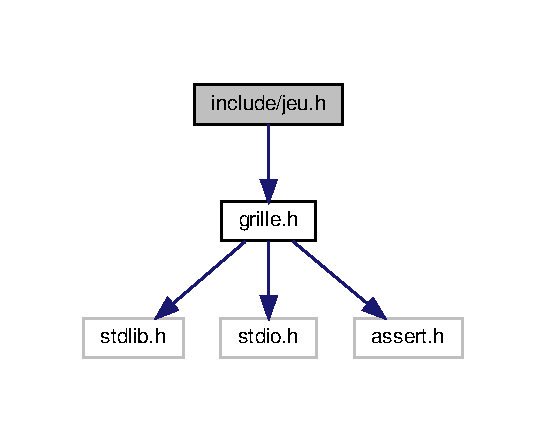
\includegraphics[width=262pt]{jeu_8h__incl}
\end{center}
\end{figure}
This graph shows which files directly or indirectly include this file\+:
\nopagebreak
\begin{figure}[H]
\begin{center}
\leavevmode
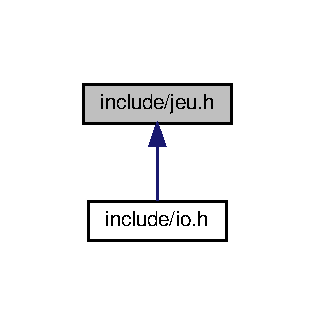
\includegraphics[width=151pt]{jeu_8h__dep__incl}
\end{center}
\end{figure}
\subsection*{Functions}
\begin{DoxyCompactItemize}
\item 
int \hyperlink{jeu_8h_adf9adf6ee75bcfbe164ac465ca5e4f82}{compte\+\_\+voisins\+\_\+vivants} (int i, int j, \hyperlink{structgrille}{grille} g)
\item 
void \hyperlink{jeu_8h_a36a600ac4a0aa461ca212614a9ba4260}{evolue} (\hyperlink{structgrille}{grille} $\ast$g, \hyperlink{structgrille}{grille} $\ast$gc, int cy)
\end{DoxyCompactItemize}


\subsection{Detailed Description}
header pour le jeu \begin{DoxyAuthor}{Author}
Marlind Tahiri 
\end{DoxyAuthor}


\subsection{Function Documentation}
\mbox{\Hypertarget{jeu_8h_adf9adf6ee75bcfbe164ac465ca5e4f82}\label{jeu_8h_adf9adf6ee75bcfbe164ac465ca5e4f82}} 
\index{jeu.\+h@{jeu.\+h}!compte\+\_\+voisins\+\_\+vivants@{compte\+\_\+voisins\+\_\+vivants}}
\index{compte\+\_\+voisins\+\_\+vivants@{compte\+\_\+voisins\+\_\+vivants}!jeu.\+h@{jeu.\+h}}
\subsubsection{\texorpdfstring{compte\+\_\+voisins\+\_\+vivants()}{compte\_voisins\_vivants()}}
{\footnotesize\ttfamily int compte\+\_\+voisins\+\_\+vivants (\begin{DoxyParamCaption}\item[{int}]{i,  }\item[{int}]{j,  }\item[{\hyperlink{structgrille}{grille}}]{g }\end{DoxyParamCaption})}

compte le nombre de voisins


\begin{DoxyParams}{Parameters}
{\em i} & nombre de lignes \\
\hline
{\em j} & nombre de colonnes \\
\hline
\end{DoxyParams}
\begin{DoxyReturn}{Returns}
{\ttfamily int} 
\end{DoxyReturn}
\mbox{\Hypertarget{jeu_8h_a36a600ac4a0aa461ca212614a9ba4260}\label{jeu_8h_a36a600ac4a0aa461ca212614a9ba4260}} 
\index{jeu.\+h@{jeu.\+h}!evolue@{evolue}}
\index{evolue@{evolue}!jeu.\+h@{jeu.\+h}}
\subsubsection{\texorpdfstring{evolue()}{evolue()}}
{\footnotesize\ttfamily void evolue (\begin{DoxyParamCaption}\item[{\hyperlink{structgrille}{grille} $\ast$}]{g,  }\item[{\hyperlink{structgrille}{grille} $\ast$}]{gc,  }\item[{int}]{cy }\end{DoxyParamCaption})}

fait evoluer la grille


\begin{DoxyParams}{Parameters}
{\em g} & grille g \\
\hline
{\em gc} & grille gc \\
\hline
{\em cy} & toggle cyclique \\
\hline
\end{DoxyParams}
\begin{DoxyReturn}{Returns}
{\ttfamily void} 
\end{DoxyReturn}

%--- End generated contents ---

% Index
\backmatter
\newpage
\phantomsection
\clearemptydoublepage
\addcontentsline{toc}{chapter}{Index}
\printindex

\end{document}
